%Suite géométrique et tableaur

\section{Efficacité d'un antibiotique (7 points)}

Un laboratoire pharmaceutique souhaite tester le temps de réaction d'un nouvel antibiotique contre le bacille de Koch responsable des tuberculoses. Pour cela, on dispose d'une culture de $10^{10}$ bactéries dans laquelle on introduit l'antibiotique. On remarque que le nombre de bactéries est divisé par quatre toutes les heures.

\subsection{\ }

On crée la feuille de calcul suivante donnant le nombre de bactéries en fonction du temps $n$ en heures.

\begin{center}
	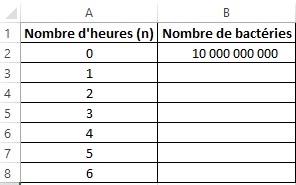
\includegraphics[scale=1]{img/bacteries}
\end{center}

\begin{questions}
	\question[1] Quelle formule faut-il enter dans la cellule \texttt{B3}, pour calculer le nombre de bactéries au bout d'une heure, de sorte qu'en recopiant cette formule vers le bas on puisse compléter les lignes suivantes.
	\begin{solution}
		Pour calculer le nombre de bactéries au bout d'une heure, on entre en $B3$ la formule suivante :
		
		\begin{equation*}
			= B2 / 4
		\end{equation*}
	\end{solution}
	
	
	\question[1]  On a recopié la formule précédente jusqu'en \texttt{B18} 
		\begin{parts}
			\part[\half] Quelle formule se trouve en \texttt{B18} ?
			\begin{solution}
				La formule en $B18$ est la suivante :
				\begin{equation*}
					= B17 / 4
				\end{equation*}
			\end{solution}
			\part[\half] Que représente concrètement la valeur calculée dans cette cellule ?
			\begin{solution}
				La valeur calculée dans cette cellule représente le nombre de bactéries 16 heures après l'introduction de l'antibiotique.
			\end{solution}
		\end{parts}
	
	
\end{questions}

\subsection{\ }

On note $u_0$ le nombre de bactéries au moment de l'injection de l'antibiotique.
Soit $(u_n)_{n \in \naturels}$, la suite représentant le nombre de bactéries, contenues dans la culture, $n$ heures après l'introduction de l'antibiotique. 

\begin{questions}
	\question[1] Exprimer $u_{n+1}$ en fonction de $u_n$.
	\begin{solution}
		Le nombre de bactéries est divisé par quatre toutes les heures, on a donc :
		\begin{eqnarray*}
			u_{n+1} &=& u_n \times \dfrac{1}{4}\\
			u_{n+1} &=& u_n \times \num{0.25}
		\end{eqnarray*}
	\end{solution}
	
	\question[1] En déduire que la suite $(u_n)$ est une suite géométrique de raison \num{0.25}.
	\begin{solution}
		Chaque terme de la suite est égal au précédent multiplié par \num{0.25}. $(u_n)$ est donc une suite géométrique de raison \num{0.25}.
	\end{solution}
	
	\question[1] Exprimer $u_n$ en fonction de $n$.
	\begin{solution}
		Expression de $u_n$ en fonction de n :
		\begin{eqnarray*}
			u_n &=& u_0 \times q^n \\
			u_n &=& 10^{10} \times \num{0.25}^n 
		\end{eqnarray*}
	\end{solution}
	
	\question[2] Calculer au bout de combien d'heures le nombre de bactéries deviendra inférieur à 100. 
	\begin{solution}
		En appliquant la formule ci-dessus, on obtient :
		\begin{eqnarray*}
			u_{13} &=& 10^{10} \times 0.25^{13} \\
			u_{13} &\approx& \num{149.01}
		\end{eqnarray*}
	
		et
		
		\begin{eqnarray*}
			u_{14} &=& 10^{10} \times 0.25^{14} \\
			u_{14} &\approx& \num{37.25}
		\end{eqnarray*}
	
	Donc le nombre de bactéries deviendra inférieur à 100 au bout de 14 heures.
	\end{solution}
\end{questions}